\documentclass[11pt]{article}
\usepackage[top=20mm,bottom=30mm,left=20mm,right=20mm]{geometry}
\usepackage[utf8]{inputenc}
\usepackage{parskip}
\usepackage{abstract}

% Biblatex
\usepackage[block=space,bibencoding=utf8,style=phys,maxbibnames=6,giveninits=true]{biblatex}
\addbibresource{../StochasticTopology.bib}

% Mathy stuff
\usepackage{physics}
\usepackage{siunitx}
\usepackage{amsmath}
\usepackage[version=4]{mhchem}

% Visual stuff
\usepackage{graphics}
\usepackage{tikz}
\usetikzlibrary{math}
\usepackage{stackengine}
\usepackage{float}

% Misc
\usepackage{hyperref}
\usepackage{cleveref}
\usepackage{lipsum}

\renewcommand{\abstractname}{}    % clear the title
\renewcommand{\absnamepos}{empty} % originally center

\setlength{\parskip}{2ex}
\setlength{\parindent}{0em}

\begin{document}
\pagenumbering{gobble}
\begin{center}
	\LARGE
	\textbf{Topological States in Out-of-Equilibrium Allosteric Assemblies} \\
	\vspace{0.3em}
	\normalsize
	\textit{Jan Kocka}
	\vspace{1em}
\end{center}

\begin{abstract}
	\small
    % General introduction to topology in biology/biophysics - 84 words
    Stochastic systems are key to many areas of biophysics as much of living matter takes place in a highly noisy environment.
    However, despite this noisiness, many biological systems show a high degree or robustness.
    A recent new direction in understanding this apparent paradox is the study of topology of stochastic systems\cite{tangTopologyProtectsChiral2021,soneHermitianNonHermitianTopology2024,zhengTopologicalMechanismRobust2024}.
    Topological states can effectively reduce the dimensionality of the configurational space and thus can explain robustness without making specific assumptions about the mechanics of a system, while themselves being robust to local changes.
    % Getting into the project - ~109 words
    In this study we look for topological features in a non-equilibrium, thermodynamically consistent stochastic model of an allosteric assembly where each unit can change conformation and (de)phosphorylate.
    The system is driven out of equilibrium by the inclusion of two different phosphorylation reactions: a direct reaction by (de)binding a phosphate group and one driven by ATP to ADP conversion.
    We allow these to couple differently depending on subunit conformation as this is to only way for an isolated subunit to favour undergoing a futile cycle of phosphorylating, changing conformation, dephosphorylating and changing conformation back.
    Such futile cycles are common in biological settings\cite{sharmaFutileCyclesEmerging2024,samoilovStochasticAmplificationSignaling2005} and give rise to topological currents when imposed artificially\cite{tangTopologyProtectsChiral2021}.
    % Getting on to results
    We find that even without explicitly favouring futile cycles in the assembly, adding a nearest neighbour interaction results in a directed probability currents in the steady state.
    % We find that even without explicitly favouring futile cycles in the assembly, adding a nearest neighbour interaction results in a directed current along boundary states which follow a collective cycle.

    % Point out that we add the locality aspect and that it is more physical

    % In particular, we drive phosphorylation via an ATP to ADP conversion at high ATP concentrations and dephosphorylation by spontaneous release of Pi.
    % In this study we consider a stochastic model for a possibly allosteric assembly 

    % Stochastic systems are key to many areas of biophysics as much of living matter is highly heterogeneous and takes place in a very noisy environment.
    % However, despite this high degree of stochasticity, many systems show a high degree or robustness and reliability.
    % A recent new direction and understanding this apparent paradox is understanding the topology of biologically relevant stochastic systems.
    % Topologically favoured states effectively reduce the dimensionality of the otherwise unrestricted space and thus can go a long way in explaining 


	% Here we study ... models ...
\end{abstract}

\vspace{1em}

\printbibliography

\vspace{1em}

\begin{figure}[H]
    \centering
    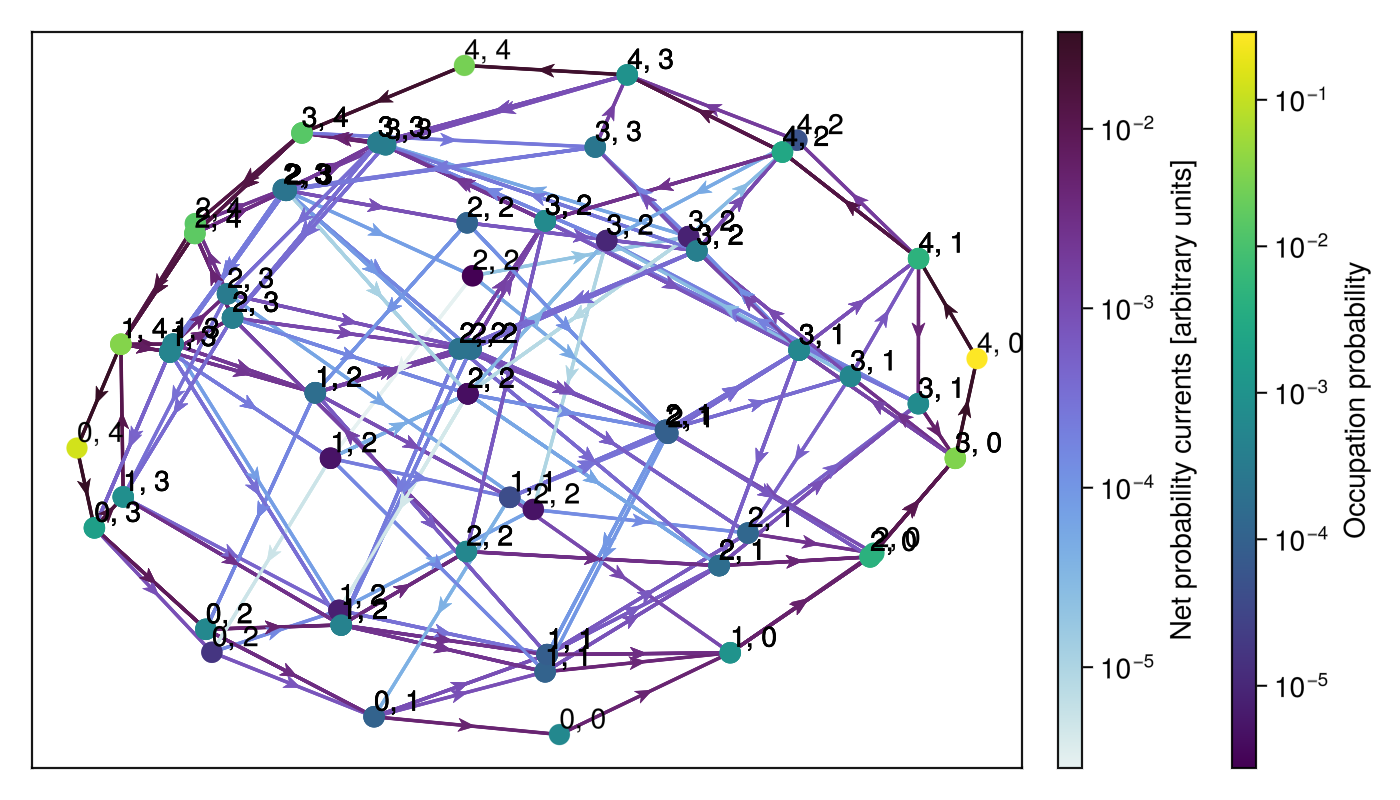
\includegraphics[width=\textwidth]{../../plots/aaa_B=1_C=2_N=4_version=2.5.png}
\end{figure}

\newpage
\section{Notes}
\subsection{Key points}
\begin{itemize}
	\item stochastic systems
	\item futile cycles
	\item non-equilibrium dynamics
	\item allostery
	\item system features
	      \begin{itemize}
		      \item complex -- high dimensional network, not pen-and-paper tractable
		      \item locality -- unlike the previous models, have NNs, can model waves along the polymer
		      \item discrete configurational space
		      \item Thermodynamically consistent? idk if this is the right wording
	      \end{itemize}
	\item Search for topological states/patterns in realistic systems (this means starting from the ground up with (non-equilibrium) statphys, LDB, no arbitrary choices) with futile cycles
	\item the futile cycle is implemented via physical parameters by coupling to two physically reasonable asymmetrical processes
\end{itemize}
\subsection{Topic?}
\begin{itemize}
	\item Perhaps the closest might be: \textbf{"Biomolecular assemblies and condensates"} given that the main model is of an allosteric assembly?
	\item Others that may be relevant:
	      \begin{itemize}
		      \item "Patterns, waves, transport, collective phenomena, and microswimmers" -- there's collective phenomena! but idk about microswimmers
		      \item "Clocks, timers and cell cycle dynamics" -- if we lean into KaiABC then maybe
		      \item "Protein structure, dynamics and interactions" -- cause I guess the polymer as I've been calling it would realistically be a protein?
		      \item "Emerging Areas in the Physics of Life" -- idk what this is but probably not
	      \end{itemize}
\end{itemize}
\subsection{"Formula"}
\paragraph{Title/Topic}
\paragraph{Motivation}
Topological phases have been a hot topic in physics ever since the quantum hall effect.
Recently their study has been extended to non-Hermitian systems such as a non-reciprocal stochastic processes.
\paragraph{Problem}
Idrk?
\paragraph{Study design}

\paragraph{Predictions and results}
\paragraph{Conclusions}

\end{document}
